\documentclass{article}
\usepackage[utf8]{inputenc}
\usepackage{graphicx}
\usepackage{tikz}

\usepackage{amsmath, amsthm, amssymb}

\usepackage{tkz-euclide}

\usepackage{gensymb}

\usetikzlibrary{calc}

\title{Notas}
\author{javalejan12 }
\date{June 2022}

\begin{document}

\maketitle

\section{Factorial}
\[
\makebox[4em]{Good:}
\hat{d}=\frac{(d+n)!}{n!\,d!}
\]
\[
\makebox[4em]{Bad:}
\hat{d}=\frac{(d+n)\,!}{n\,!d\,!}
\]

\section{Sector circular}
\centering
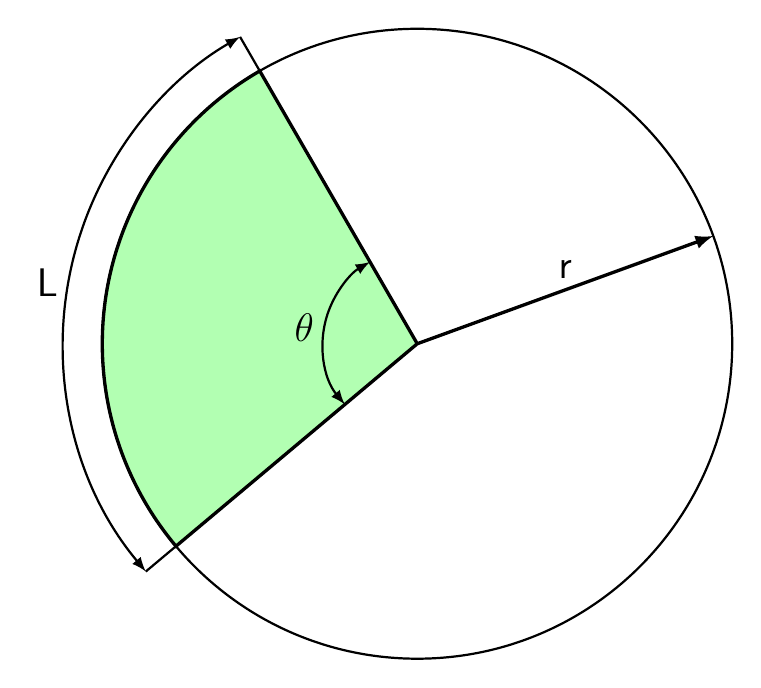
\begin{tikzpicture}[thick,font=\sffamily\Large]
\draw (0,0) circle (4cm);
\draw[very thick,fill=green!30] (0,0) --  (220:4) arc(220:120:4) -- cycle;
\draw[latex-latex]  (220:1.2) arc(220:120:1.2) node[midway,left]{$\theta$};
\draw[latex-latex]  (220:4.5) arc(220:120:4.5) node[midway,left]{L};
\draw (120:4) -- (120:4.5) (220:4) -- (220:4.5);
\draw[very thick,-latex] (0,0) --  (20:4) node[midway,above]{r};
\end{tikzpicture}


\end{document}
